The Higgs boson ($H$) was discovered at the Large Hadron Collider (LHC) in 2012, by the ATLAS and CMS
collaborations \cite{HIGG-2012-27,CMS-HIG-12-028}.
All current measurements of its spin and couplings \cite{HIGG-2013-02,HIGG-2013-17,CMS-HIG-13-033,CMS-HIG-13-002,CMS-HIG-13-023}
are so far consistent with the Standard Model (SM) predictions \cite{PhysRevLett.13.321,HIGGS1964132,PhysRevLett.13.508,PhysRev.145.1156,PhysRevLett.13.585,PhysRev.155.1554}.
The measured mass of the Higgs boson is 125.09 $\pm$ 0.21 (stat.) $\pm$ 0.11 (syst.) $\GeV$ \cite{HIGG-2014-14}.

One of the primary physics goals for the High Luminosity LHC (HL-LHC) and beyond is to measure the Higgs boson trilinear self-coupling (\hhh), which is directly related to the shape of the Higgs potential, and therefore it is essential for probing the exact nature of the Higgs mechanism and electroweak symmetry breaking. It is expected that the self-coupling of the Higgs boson can be experimentally established by measuring the Higgs boson pair production ($HH$). In the SM, pairs of Higgs bosons at the LHC are dominantly produced in gluon-gluon fusion ($gg$F) processes, namely via a loop of top quarks (“box diagram”) and the Higgs self-interaction (“triangle diagram”), as shown in Figures~\ref{fig:BoxDiagram} and \ref{fig:TriangleDiagram}, respectively.

\begin{figure}[!h]
\centering
\captionsetup[subfigure]{justification=centering}
\subfloat[$HH$ production via the top-quark Yukawa coupling\label{fig:BoxDiagram}]{      % first box diagram *****************************************
\begin{tikzpicture}
\begin{feynman}
\vertex (a) {\(g\)};
\vertex [right=1.5cm of a] (t1);
\vertex [right=1.5cm of t1, large, dot, blue] (t2) {};
\vertex [below=1.5cm of t1] (t3);
\vertex [left=1.5cm of t3, below=of a] (b) {\(g\)};
\vertex [right=1.5cm of t3, below=of t2, large, dot, blue] (t4) {};
\vertex [right=1.5cm of t2] (h1) {\(H\)};
\vertex [right=1.5cm of t4] (h2) {\(H\)};
\diagram* {
(t2) -- [fermion,line width=0.35mm] (t1) -- [gluon,line width=0.35mm] (a),
(t1) -- [fermion,line width=0.35mm] (t3),
(t3) -- [gluon,line width=0.35mm] (b),
(t3) -- [fermion,line width=0.35mm] (t4),
(t4) -- [fermion,line width=0.35mm] (t2),
(t2) -- [dashed,line width=0.35mm] (h1),
(t4) -- [dashed,line width=0.35mm] (h2),
};
\vertex [right=0.45cm of t2] (t2note);
\vertex [below=0.1cm of t2note, blue] (t2note1) {\(y_{ttH}\)};
\end{feynman}
\end{tikzpicture} 
%}%subfig 
%\subfloat[]{ %      second box diagram *****************************************
\hspace{0.2cm}
\begin{tikzpicture}
\begin{feynman}
\vertex (a) {\(g\)};
\vertex [right=1.5cm of a] (t1);
\vertex [below=0.75cm of t1] (t1p);
\vertex [right=1.5cm of t1, large, dot, blue] (t2) {};
\vertex [below=1.5cm of t1] (t3);
\vertex [above right=0.36cm of t3] (t3p);
\vertex [left=1.5cm of t3, below=of a] (b) {\(g\)};
\vertex [right=1.5cm of t3, below=of t2, large, dot, blue] (t4) {};
\vertex [below=0.75cm of t2] (t5);
\vertex [right=1.5cm of t2] (h1) {\(H\)};
\vertex [right=1.5cm of t4] (h2) {\(H\)};
\diagram* {
(a) -- [gluon,line width=0.35mm] (t5),
(t3p) -- [gluon,line width=0.35mm] (b),
(t5) -- [fermion,line width=0.35mm] (t2),
(t4) -- [fermion,line width=0.35mm] (t5),
(t2) -- [dashed,line width=0.35mm] (h1),
(t4) -- [dashed,line width=0.35mm] (h2),
(t2) -- [fermion,line width=0.35mm, out=180, in=90] (t1p),
(t1p) -- [fermion,line width=0.35mm, in=180, out=-90] (t4),
%(t3p) -- [plain,line width=0.35mm, in=180, out=160] (t2),
};
\end{feynman}
\end{tikzpicture} 
}%subfig 
%\qquad
\hspace{0.1cm}
\subfloat[$HH$ production via the Higgs boson self-coupling\label{fig:TriangleDiagram}]{     % self-coupling diagram *****************************************
\hspace{0.2cm}
\begin{tikzpicture}
\begin{feynman}
\vertex (a) {\(g\)};
\vertex [below=1.5cm of a] (b) {\(g\)};
\vertex [right=1.5cm of a] (t1);
\vertex [right=1.5cm of b] (t2);
\vertex [right=1.2cm of t1] (t1p);
\vertex [below=0.75cm of t1p] (t3m);
\vertex [right=0.01cm of t3m, large, dot, blue] (t3) {};
\vertex [right=1.5cm of t3, large, dot, red] (h1) {};
\vertex [right=2.65cm of t1p] (h2);
\vertex [right=3.85cm of t2] (h3);
\vertex [right=0.01cm of h2] (h2p) {\(H\)};
\vertex [right=0.01cm of h3] (h3p) {\(H\)};
\diagram* {
(a) -- [gluon,line width=0.35mm] (t1),
(b) -- [gluon,line width=0.35mm] (t2),
(t1) -- [fermion,line width=0.35mm] (t2),
(t2) -- [fermion,line width=0.35mm] (t3),
(t3) -- [fermion,line width=0.35mm] (t1),
(t3) -- [dashed,line width=0.35mm, edge label'=\(H\)] (h1),
(h1) -- [dashed,line width=0.35mm] (h2),
(h1) -- [dashed,line width=0.35mm] (h3),
};
\vertex [above=0.4cm of h1] (l);
\vertex [left=-0.3cm of l, red] {\(\lambda_{HHH}\)};
\end{feynman}
\end{tikzpicture} \ \ \
}%subfig 
        \caption{Leading-order Feynman diagrams for the $gg$F pair production of Higgs bosons in the SM. The vertices represented by the blue dots correspond to top-quark Yukawa interactions ($y_{ttH}$), while the vertex represented by the red dot corresponds to the trilinear Higgs boson self-coupling (\hhh).}
        \label{fig:HHProductionFeynmanDiagrams}
    \end{figure}

Due to the destructive interference between the box and triangle diagrams, the cross-section of the pair production of Higgs bosons in the SM is very small (31.05$^{+6.0\%}_{-23.0\%}$ (scale+mtop scheme) $\pm$ 3.0\% (PDF+$\alpha_{\mathrm{S}}$)~fb at $\rts~= \SI{13} \TeV$ \cite{Grazzini:2018bsd}), about 1000 times smaller than the single Higgs boson production cross-section. 

\begin{figure}
\centering
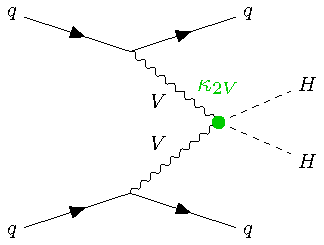
\includegraphics[width=.3\textwidth]{figures/intro_diagrams/VBF_k2v.pdf}
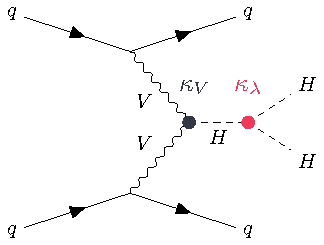
\includegraphics[width=.3\textwidth]{figures/intro_diagrams/VBF_kvkl.pdf}
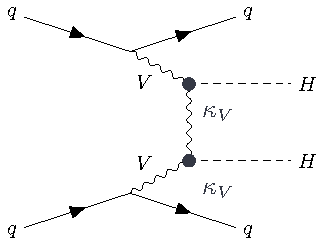
\includegraphics[width=.3\textwidth]{figures/intro_diagrams/VBF_kvkv.pdf}
\caption{Tree-level Feynman diagrams for the non-resonant VBF $HH$ production. The vertices denoted by $\kappa_{2V}$, $\kappa_{V}$ and $\kappa_{\lambda}$ represent the $VVHH$, $VVH$ and $HHH$ couplings, respectively.}
\label{fig:VBFfeynman}
\end{figure}

The cross-section of the pair production of Higgs bosons via the vector boson production (VBF) in the SM is even smaller: 1.726$^{+0.03\%}_{-0.04\%}$ (scale) $\pm$ 2.1\% (PDF+$\alpha_{\mathrm{S}}$)~fb at $\rts~= \SI{13} \TeV$ \cite{Dreyer_2018}. The tree-level diagrams for the VBF HH process are shown in Figure \ref{fig:VBFfeynman}.

Thus, the SM $HH$ production is not expected to be observed with the data so far collected by the ATLAS experiment.  However, a variety of new physics models predict enhancements to this cross-section. Modifications of the Higgs top-quark Yukawa coupling or modifications of the Higgs self-coupling, or presence of new diagrams with new couplings could enhance the non-resonant di-Higgs production cross section. Therefore, a search for Higgs pair production with current data is a probe of new physics. 

Theories beyond the SM (BSM) predict heavy resonances that could decay into a pair of the SM Higgs bosons, such as a heavy spin-0 scalar $X$ in two-Higgs-doublet models (2HDM) \cite{Branco:2011iw,}, as shown in Figure~\ref{fig:ResonantggFPairProduction}. The presence of such resonances would also enhance the di-Higgs production cross section.  %and spin-2 Kaluza Klein (KK) excitations of the graviton G$^{*}_{\mathrm{KK}}$, in the bulk Randall-Sundrum (RS) model \cite{PhysRevD.76.036006,Fitzpatrick_2007}.

\begin{figure}[!h]
\centering
\begin{tikzpicture}
\begin{feynman}
\vertex (a);
\vertex [below=1.5cm of a] (b);
\vertex [left=0.01cm of a] (ap) {\(g\)};
\vertex [left=0.01cm of b] (bp) {\(g\)};
\vertex [right=1.2cm of a] (t1);
\vertex [below=0.75cm of t1] (v1x);
\vertex [right=0.01cm of v1x, blob] (v1) {};
\vertex [right=1.2cm of v1] (v2);
\vertex [right=1.2cm of v2] (f1);
\vertex [above=0.75cm of f1] (f2);
\vertex [below=0.75cm of f1] (f3);
\vertex [right=0.01cm of f2] (f2p) {\(H\)};
\vertex [right=0.01cm of f3] (f3p) {\(H\)};
\diagram* {
(a) -- [gluon,line width=0.35mm] (v1),
(v1) -- [gluon,line width=0.35mm] (b),
(v1) -- [dashed,line width=0.35mm, edge label'=\(X\)] (v2),
(v2) -- [dashed,line width=0.35mm] (f2),
(v2) -- [dashed,line width=0.35mm] (f3),
};
\end{feynman}
\end{tikzpicture}
\caption{Feynman diagram corresponding to BSM $gg$F resonant pair production of the SM Higgs bosons. The patterned-background circle indicates an effective coupling of the hypothetical resonance $X$ to gluons.}
\label{fig:ResonantggFPairProduction}
\end{figure}

This note describes searches for non-resonant and resonant $HH$ production in a final state with two $b$-jets and two $\tau$ leptons using 139~\ifb\ of 
13~TeV $pp$ collision data recorded by the ATLAS experiment between 2015 and 2018. The \bbtt channel has the third largest branching fraction (7.3\%) of the experimentally feasible channels and it represents 
a relatively clean final state compared to the channels with larger branching fractions (\bbbb and $\bbbar\Wplus\Wminus$) due to a better separation from the multijet and \ttbar backgrounds. Since $\tau$ leptons 
can decay either leptonically ($\tau_{\mathrm{lep}}$: into electrons, $e$, or muons, $\mu$) or hadronically ($\tau_{\mathrm{had}}$: typically into one or three charged pions, plus some number of neutral pions), 
both \lephad and \hadhad decay channels are considered, where each subscript indicates the decay mode of the corresponding $\tau$ lepton. Parametric neural networks (PNN) are used to provide optimal 
separation between resonant signal and background processes and to improve the sensitivity to the different signal models. The BDT(NN) algorithm is used to separate the non-resonant signal and the backgrounds for the \hadhad (\lephad) channel.

Previously, searches for $HH$ production in the \bbtt channel were performed by the ATLAS experiment using 20.3~\ifb\ of
8~TeV $pp$ collision data (only \lephad decay mode was considered)~\cite{HIGG-2013-33} and using 36.1~\ifb\ of 13~TeV $pp$ collision data~\cite{HIGG-2016-16}. Separate searches have been performed in the $\bbbar\Wplus\Wminus$~\cite{HIGG-2016-27},
$\bbbar\bbbar$~\cite{EXOT-2016-31}, $\yybb$~\cite{HIGG-2016-15}, $\Wplus\Wminus\Wplus\Wminus$~\cite{HIGG-2016-24}, 
and $\Wplus\Wminus\gamma\gamma$~\cite{HIGG-2016-20} final states using up to 36.1~\ifb\ of 13~TeV $pp$ collision data. A statistical combination of these results and those obtained for the \bbtt\ channel for the same centre-of-mass energy has been reported as well~\cite{HDBS-2018-58}. A search for non-resonant $HH$ production in $bb\ell\nu\ell\nu$ was also performed using 139~\ifb\ of 13~TeV $pp$ collision data~\cite{Aad_2020}.

Searches for resonant Higgs boson pair production in the \bbtt channel were performed also by the CMS experiment, using 18.3~\ifb\ of 8~TeV $pp$ collision data~\cite{PhysRevD.96.072004} and using 35.9~\ifb\ of 13~TeV $pp$ collision data~\cite{Sirunyan:2017djm}.

This analysis contains various improvements with respect to the previous publication:
\begin{itemize}
\item looser $b$-tagging working point (77\% vs 70\%) at the same background rejection efficiency;
\item improvements in the \tauhad reconstruction due to improved track selection (6-10\% relative improvement in the reconstruction efficiency);
\item BDT-based \tauhad-eVeto instead of likelihood-based method;
\item RNN-\tauhad ID instead of BDT-based (13-25\% relative efficiency improvement);
\item PNN instead of BDT for the resonant signal for \lephad and \hadhad channels;
\item NN for \lephad non-resonant channel with improved signal/background separation;
\item new fake background estimate methods for the \hadhad channel;
\item larger data set.
\end{itemize}
That results in about a factor of 2 better limits on top of the increase in the luminosity.